% Anonymized submission build. Comment out the next line for the named version.
\def\anonymous{}
%% Submission to Engineering Applications of Artificial Intelligence (Elsevier), elsarticle single-column preprint layout.
%% Overleaf: upload main.tex, numbers.tex, tab_*.tex, refs.bib, figures/, elsarticle.cls, elsarticle-num.bst.
%% Colour conventions:  \pend{...} (red) open item;  \proj{...} (blue) model-based projection or hypothesis, not a measurement.
%% Revision of 8 Nov 2026:  \add{...} (blue) added text;  \del{...} (blue, struck through) deleted text;  \maskred{...} (red) feedback-mask passages for the authors.
\documentclass[preprint,12pt,times]{elsarticle}
\usepackage{amsmath,amssymb}
\usepackage{graphicx}
\usepackage{booktabs}
\usepackage{xcolor}
\makeatletter
\IfFileExists{ulem.sty}{\usepackage[normalem]{ulem}}{%
  % fallback strike-out (word by word) when ulem is not installed; Overleaf uses ulem
  \def\sout##1{\sout@w##1 \@nil}%
  \def\sout@w##1 ##2\@nil{\sout@one{##1}\ifx\relax##2\relax\else\ \sout@w##2\@nil\fi}%
  \def\sout@one##1{\leavevmode\setbox0\hbox{##1}\rlap{\rule[0.55ex]{\wd0}{0.4pt}}\box0}}
\makeatother
\usepackage[ruled,linesnumbered,vlined]{algorithm2e}
\usepackage{siunitx}
\usepackage{tikz}
\usetikzlibrary{positioning,arrows.meta,fit,calc}
\usepackage{microtype}
\usepackage[hidelinks]{hyperref}
\newcommand{\pend}[1]{\textcolor{red}{[#1]}}
\newcommand{\proj}[1]{\textcolor{blue}{#1}}
\newcommand{\add}[1]{{\color{blue}#1}}
\newcommand{\del}[1]{\textcolor{blue}{\sout{#1}}}
\newcommand{\maskred}[1]{\textcolor{red}{#1}}
\definecolor{harel}{RGB}{0,140,60}
\newcommand{\hadd}[1]{{\color{harel}#1}}
\newcommand{\hdel}[1]{\textcolor{harel}{\sout{#1}}}
\newcommand{\hnote}[1]{\textcolor{harel}{[Harel: #1]}}

\newcommand{\ninc}{n_{\mathrm{inc},j}}
\input{numbers}
\input{numbers_rule}
\input{numbers_controls}
\newcommand{\ctlRbothallW}{18}
\newcommand{\ctlRbothallL}{8}
\newcommand{\ctlRbothallPos}{29}
\newcommand{\ctlRbothallN}{45}
\newcommand{\ctlRbothallMed}{+2.00}
\newcommand{\ctlRbothsparseW}{18}
\newcommand{\ctlRbothsparseL}{0}
\newcommand{\ctlRbothsparsePos}{28}
\newcommand{\ctlRbothsparseN}{32}
\newcommand{\ctlRbothsparseMed}{+3.96}
\newcommand{\ctlRbothdenseW}{0}
\newcommand{\ctlRbothdenseL}{8}
\newcommand{\ctlRbothdensePos}{1}
\newcommand{\ctlRbothdenseN}{13}
\newcommand{\ctlRbothdenseMed}{$-$5.43}
\newcommand{\ctlQbothallW}{8}
\newcommand{\ctlQbothallL}{2}
\newcommand{\ctlQbothallPos}{18}
\newcommand{\ctlQbothallN}{45}
\newcommand{\ctlQbothallMed}{$-$0.51}
\newcommand{\ctlQbothsparseW}{4}
\newcommand{\ctlQbothsparseL}{2}
\newcommand{\ctlQbothsparsePos}{9}
\newcommand{\ctlQbothsparseN}{32}
\newcommand{\ctlQbothsparseMed}{$-$1.29}
\newcommand{\ctlQbothdenseW}{4}
\newcommand{\ctlQbothdenseL}{0}
\newcommand{\ctlQbothdensePos}{9}
\newcommand{\ctlQbothdenseN}{13}
\newcommand{\ctlQbothdenseMed}{+0.95}
\newcommand{\ctlBbothallW}{4}
\newcommand{\ctlBbothallL}{2}
\newcommand{\ctlBbothallPos}{20}
\newcommand{\ctlBbothallN}{45}
\newcommand{\ctlBbothallMed}{$-$0.54}
\newcommand{\ctlBbothsparseW}{0}
\newcommand{\ctlBbothsparseL}{2}
\newcommand{\ctlBbothsparsePos}{10}
\newcommand{\ctlBbothsparseN}{32}
\newcommand{\ctlBbothsparseMed}{$-$1.33}
\newcommand{\ctlBbothdenseW}{4}
\newcommand{\ctlBbothdenseL}{0}
\newcommand{\ctlBbothdensePos}{10}
\newcommand{\ctlBbothdenseN}{13}
\newcommand{\ctlBbothdenseMed}{+0.95}
\newcommand{\ctlrulebothallW}{3}
\newcommand{\ctlrulebothallL}{2}
\newcommand{\ctlrulebothallPos}{7}
\newcommand{\ctlrulebothallN}{12}
\newcommand{\ctlrulebothallMed}{+0.85}
\newcommand{\ctlrulebothsparseW}{2}
\newcommand{\ctlrulebothsparseL}{1}
\newcommand{\ctlrulebothsparsePos}{4}
\newcommand{\ctlrulebothsparseN}{6}
\newcommand{\ctlrulebothsparseMed}{+8.52}
\newcommand{\ctlrulebothdenseW}{1}
\newcommand{\ctlrulebothdenseL}{1}
\newcommand{\ctlrulebothdensePos}{3}
\newcommand{\ctlrulebothdenseN}{6}
\newcommand{\ctlrulebothdenseMed}{+0.17}
\newcommand{\ctlSRbothallW}{2}
\newcommand{\ctlSRbothallL}{3}
\newcommand{\ctlSRbothallPos}{5}
\newcommand{\ctlSRbothallN}{12}
\newcommand{\ctlSRbothallMed}{$-$0.67}
\newcommand{\ctlSRbothsparseW}{2}
\newcommand{\ctlSRbothsparseL}{1}
\newcommand{\ctlSRbothsparsePos}{4}
\newcommand{\ctlSRbothsparseN}{6}
\newcommand{\ctlSRbothsparseMed}{+8.52}
\newcommand{\ctlSRbothdenseW}{0}
\newcommand{\ctlSRbothdenseL}{2}
\newcommand{\ctlSRbothdensePos}{1}
\newcommand{\ctlSRbothdenseN}{6}
\newcommand{\ctlSRbothdenseMed}{$-$1.26}
\newcommand{\ctlSQbothallW}{1}
\newcommand{\ctlSQbothallL}{6}
\newcommand{\ctlSQbothallPos}{3}
\newcommand{\ctlSQbothallN}{12}
\newcommand{\ctlSQbothallMed}{$-$6.08}
\newcommand{\ctlSQbothsparseW}{0}
\newcommand{\ctlSQbothsparseL}{5}
\newcommand{\ctlSQbothsparsePos}{0}
\newcommand{\ctlSQbothsparseN}{6}
\newcommand{\ctlSQbothsparseMed}{$-$18.64}
\newcommand{\ctlSQbothdenseW}{1}
\newcommand{\ctlSQbothdenseL}{1}
\newcommand{\ctlSQbothdensePos}{3}
\newcommand{\ctlSQbothdenseN}{6}
\newcommand{\ctlSQbothdenseMed}{+0.17}
\newcommand{\ctlSoneRuleBothW}{22}
\newcommand{\ctlSoneRuleBothL}{0}
\newcommand{\ctlSoneRuleBothPos}{37}
\newcommand{\ctlSoneRuleBothN}{45}
\newcommand{\ctlruleBothSignP}{0.39}
\newcommand{\ctlruleBothPos}{7}
\newcommand{\ctlruleBothN}{12}
\newcommand{\ctlRselfSW}{7}
\newcommand{\ctlRselfSL}{0}
\newcommand{\ctlRselfSPos}{31}
\newcommand{\ctlRselfSN}{45}
\newcommand{\ctlRselfSMed}{+1.37}
\newcommand{\ctlQselfSW}{8}
\newcommand{\ctlQselfSL}{0}
\newcommand{\ctlQselfSPos}{19}
\newcommand{\ctlQselfSN}{45}
\newcommand{\ctlQselfSMed}{+0.00}
\newcommand{\ctlQRRW}{4}
\newcommand{\ctlQRRL}{7}
\newcommand{\ctlQRRPos}{17}
\newcommand{\ctlQRRN}{45}
\newcommand{\ctlQRRMed}{$-$0.73}
\newcommand{\selFiveROneN}{45}
\newcommand{\selFiveROneChanged}{33}
\newcommand{\selFiveROneSlow}{33}
\newcommand{\selFiveQOneN}{45}
\newcommand{\selFiveQOneChanged}{24}
\newcommand{\selFiveQOneSlow}{24}
\newcommand{\selFiveQROneN}{45}
\newcommand{\selFiveQROneChanged}{27}
\newcommand{\selFiveQROneSlow}{27}
\newcommand{\selFiveRTwoN}{12}
\newcommand{\selFiveRTwoChanged}{6}
\newcommand{\selFiveRTwoSlow}{6}
\newcommand{\selFiveQTwoN}{12}
\newcommand{\selFiveQTwoChanged}{8}
\newcommand{\selFiveQTwoSlow}{8}
\newcommand{\noLROneN}{45}
\newcommand{\noLROneW}{0}
\newcommand{\noLROneL}{36}
\newcommand{\noLROneMed}{$-$40.50}
\newcommand{\noLROneWithin}{2}
\newcommand{\noLROnePos}{0}
\newcommand{\noLROneIncL}{50.9}
\newcommand{\noLROneIncN}{4349.6}
\newcommand{\noLROneWorks}{no}
\newcommand{\noLROneTmW}{0}
\newcommand{\noLROneTmL}{40}
\newcommand{\noLROneTmMed}{$-$34.59}
\newcommand{\noLROneSparseMed}{$-$44.66}
\newcommand{\noLROneSparseL}{27}
\newcommand{\noLROneSparseN}{32}
\newcommand{\noLROneSparseWithin}{0}
\newcommand{\noLROneDenseMed}{$-$18.33}
\newcommand{\noLROneDenseL}{9}
\newcommand{\noLROneDenseN}{13}
\newcommand{\noLROneDenseWithin}{2}
\newcommand{\noLQOneN}{45}
\newcommand{\noLQOneW}{0}
\newcommand{\noLQOneL}{28}
\newcommand{\noLQOneMed}{$-$31.69}
\newcommand{\noLQOneWithin}{3}
\newcommand{\noLQOnePos}{0}
\newcommand{\noLQOneIncL}{28.4}
\newcommand{\noLQOneIncN}{2542.2}
\newcommand{\noLQOneWorks}{no}
\newcommand{\noLQOneTmW}{0}
\newcommand{\noLQOneTmL}{26}
\newcommand{\noLQOneTmMed}{$-$30.71}
\newcommand{\noLQOneSparseMed}{$-$35.42}
\newcommand{\noLQOneSparseL}{19}
\newcommand{\noLQOneSparseN}{32}
\newcommand{\noLQOneSparseWithin}{0}
\newcommand{\noLQOneDenseMed}{$-$25.25}
\newcommand{\noLQOneDenseL}{9}
\newcommand{\noLQOneDenseN}{13}
\newcommand{\noLQOneDenseWithin}{3}
\newcommand{\noLRTwoN}{12}
\newcommand{\noLRTwoW}{0}
\newcommand{\noLRTwoL}{10}
\newcommand{\noLRTwoMed}{$-$45.11}
\newcommand{\noLRTwoWithin}{0}
\newcommand{\noLRTwoPos}{0}
\newcommand{\noLRTwoIncL}{65.7}
\newcommand{\noLRTwoIncN}{1900.3}
\newcommand{\noLRTwoWorks}{no}
\newcommand{\noLRTwoTmW}{0}
\newcommand{\noLRTwoTmL}{12}
\newcommand{\noLRTwoTmMed}{$-$43.66}
\newcommand{\noLRTwoSparseMed}{$-$43.33}
\newcommand{\noLRTwoSparseL}{4}
\newcommand{\noLRTwoSparseN}{6}
\newcommand{\noLRTwoSparseWithin}{0}
\newcommand{\noLRTwoDenseMed}{$-$45.11}
\newcommand{\noLRTwoDenseL}{6}
\newcommand{\noLRTwoDenseN}{6}
\newcommand{\noLRTwoDenseWithin}{0}
\newcommand{\noLQTwoN}{12}
\newcommand{\noLQTwoW}{0}
\newcommand{\noLQTwoL}{4}
\newcommand{\noLQTwoMed}{$-$7.41}
\newcommand{\noLQTwoWithin}{1}
\newcommand{\noLQTwoPos}{1}
\newcommand{\noLQTwoIncL}{23.1}
\newcommand{\noLQTwoIncN}{1259.9}
\newcommand{\noLQTwoWorks}{no}
\newcommand{\noLQTwoTmW}{0}
\newcommand{\noLQTwoTmL}{9}
\newcommand{\noLQTwoTmMed}{$-$15.68}
\newcommand{\noLQTwoSparseMed}{$-$11.37}
\newcommand{\noLQTwoSparseL}{1}
\newcommand{\noLQTwoSparseN}{6}
\newcommand{\noLQTwoSparseWithin}{1}
\newcommand{\noLQTwoDenseMed}{$-$7.41}
\newcommand{\noLQTwoDenseL}{3}
\newcommand{\noLQTwoDenseN}{6}
\newcommand{\noLQTwoDenseWithin}{0}
\newcommand{\fiveTuneRuns}{421}
\newcommand{\fiveTestRuns}{832}

\setlength{\emergencystretch}{1.5em}
\pdfinfoomitdate=1
\pdftrailerid{}
\journal{Engineering Applications of Artificial Intelligence}

\begin{document}
\begin{frontmatter}
\title{Qualified-majority clauses and targeted forgetting for clause-constrained Tsetlin machines on associative processors}

\ifdefined\anonymous
\author{Anonymous authors}
\else
\author[biu]{Harel Shrot}
\author[biu]{Leonid Yavits\corref{cor1}}
\cortext[cor1]{Corresponding author.}
\affiliation[biu]{organization={Faculty of Engineering and EnICS Labs, Bar-Ilan University},
  city={Ramat Gan}, country={Israel}}
\fi

\begin{abstract}
In-memory Tsetlin machine (TM) accelerators store one clause per row, so the clause budget sets the array area and energy.
The contribution in artificial intelligence is two learning modifications for small clause budgets.
Qualified-majority (QM) clauses fire when at most a fixed fraction of their included literals is violated.
Targeted forgetting (R1) restricts the Type~Ib feedback of a non-firing clause to literals that are false on the sample.
The application in engineering is in-memory TM hardware.
On an associative-processor TM, QM uses the threshold of an approximate-search content-addressable memory, and R1 adds one compared bit.
\proj{Projected inference latency is unchanged, and training needs 36 to 44\,\% more cycles than the original design.}
We evaluate both on 19 public datasets with protocols fixed in advance and Holm-corrected Welch tests.
Against the vanilla TM as first tuned, R1 wins \numRwin{} of 48 cells, all on sparse text, and a density rule (R1 below \SI{3}{\percent} density, QM above) wins \numruleWin{} of \numruleN{} cells on six unseen datasets without a loss.
\del{A control then strengthened only the vanilla TM by lowering its specificity and literal budget.}
\del{Against it, R1 still wins \ctlRextsparseW{} sparse cells by 3.0 to 11.7 percentage points (pp) and loses \ctlRextsparseL{}.}
\del{The best QM-family arm beats the better of this baseline and R1 in \ctlBextdenseW{} dense cells by 1.2 to 5.5~pp and loses in \ctlBextdenseL{}.}
\del{Out of sample, the density rule is not confirmed (\ctlruleextallW{} wins, \ctlruleextallL{} losses).}
\del{The baseline tuning grid matters more than either modification.}
\add{Controls then lowered the specificity and literal budget of the vanilla TM and the specificity of R1 and QM.
With all arms re-tuned, R1 wins \ctlRbothsparseW{} sparse cells by 1.5 to 17.2 percentage points (pp) and loses \ctlRbothdenseL{} dense cells.
QM wins \ctlQbothallW{} cells by 1.2 to 10.9~pp and loses \ctlQbothallL{}.
Out of sample, the density rule is not confirmed (\ctlrulebothallW{} wins, \ctlrulebothallL{} losses).
Neither R1 nor QM works without the literal budget.
Unequal tuning grids changed the conclusions more than either modification did.}
\end{abstract}

\begin{keyword}
Tsetlin machine \sep associative processor \sep content-addressable memory \sep approximate search \sep in-memory computing \sep interpretable machine learning
\end{keyword}
\end{frontmatter}

%% ---------------------------------------------------------------------------
\section{Introduction}
\label{sec:intro}

The Tsetlin machine (TM)~\cite{granmo2018tm} classifies with conjunctive clauses of Boolean literals, learned by teams of finite-state automata.
Its inference uses only AND, NOT and counting.
This makes it a natural fit for in-memory hardware, where a clause maps to one memory line and is evaluated in place~\cite{ghazal2025impact,shrot2026aptm}.
AP(TM)~\cite{shrot2026aptm} implements both training and inference of a TM on an associative processor (AP)~\cite{yavits2015ap}.
It evaluates all clauses with one compare and updates all selected clauses with parallel writes.
Its latency therefore depends only weakly on the number of clauses.
Its area and energy are not: every clause occupies a row, and every compare and write activates every row.

The clause budget is thus the main hardware cost of an in-memory TM.
A standard TM, however, needs many clauses.
A clause either fires or does not, and a single violated literal silences it.
With few clauses per class, a TM loses accuracy because each clause must be specific enough to avoid false positives and general enough to fire on unseen samples.

This paper asks whether two simple modifications can recover accuracy at small clause budgets without changing the hardware substantially, and how robust any gain is to the tuning of the vanilla baseline.
\begin{itemize}
\item \textbf{Qualified-majority (QM) clauses.} A clause fires when at most a fraction $1-\theta$ of its included literals is violated. The vanilla TM is the case $\theta = 1$.
\item \textbf{Targeted forgetting (R1).} When a clause of the target polarity does not fire, standard Type~Ib feedback moves every automaton of the clause toward exclusion with probability $1/s$. R1 applies this forgetting only to the literals that are false on the sample, and leaves the satisfied literals untouched.
\end{itemize}

The two rules suit an associative processor well.
QM clause evaluation is a Hamming-distance-tolerant search, which approximate-search CAMs support with a programmable threshold~\cite{garzon2022hdcam,garzon2025jssc}.
R1 conditions an existing feedback write on the input bit, which the AP already broadcasts.

\textbf{Contributions.}
\begin{enumerate}
\item We define relative QM clauses, a polarity-aware variant, and R1, and we combine them with the literal budget of~\cite{abeyrathna2023csc} (Section~\ref{sec:method}).
\item We map QM\add{, QP} and R1 onto AP(TM) with an approximate-search CAM, and we project the cost with the analytical model of~\cite{shrot2026aptm} (Section~\ref{sec:hw}).
\item We evaluate all combinations against the vanilla TM with protocols fixed in advance, on 13 public datasets and 20 encodings from \SI{0.34}{\percent} to \SI{54}{\percent} input density, with five test seeds per arm and family-wise error control. We then test a density rule, R1 below \SI{3}{\percent} input density and QM above, on six further datasets (Sections~\ref{sec:setup} to~\ref{sec:res-rule}).
\item We repeat every contrast against a stronger vanilla TM, tuned over a smaller specificity value and a smaller literal budget (Section~\ref{sec:res-base}), and we re-tune it in a budget sweep up to 160 clauses per class (Section~\ref{sec:res-budget}). \del{The modified arms are not re-tuned. Most of the original R1 gains vanish.} \add{Re-tuning only the vanilla TM removes most of the original R1 gains. Offering the same specificity to R1 and QM restores most of them (Section~\ref{sec:res-base}).} R1 keeps significant gains on sparse many-class text and QM on dense image and signal data, but the density rule is not confirmed out of sample. \add{An ablation shows that neither modification works without the literal budget (Section~\ref{sec:res-noL}).} We report these negative results in full.
\end{enumerate}

%% ---------------------------------------------------------------------------
\section{Background}
\label{sec:bg}

\subsection{Tsetlin machine}
A TM for $K$ classes and $n$ Boolean features uses $M = 2n$ literals, the features and their negations.
Each class has $C$ clauses, half of positive and half of negative polarity.
Each clause $j$ owns one Tsetlin automaton (TA) per literal.
A TA with $2^N$ states includes its literal in the clause in the upper half of its states and excludes it in the lower half.
Clause $j$ outputs
\begin{equation}
o_j = \bigwedge_{k \in I_j} \ell_k,
\label{eq:and}
\end{equation}
where $I_j$ is the set of included literals and $\ell_k$ the value of literal $k$ on the sample.
The class score is the number of firing positive clauses minus the number of firing negative clauses.
The prediction is the class with the highest score.

Training presents each sample to its target class and to one randomly drawn other class~\cite{granmo2018tm,pytsetlinmachine}.
Each clause of these classes receives feedback with a probability that falls as the class score approaches a margin $T$.
Type~I feedback goes to clauses whose polarity agrees with the sample's membership in the class.
If such a clause fires, Type~Ia moves the TAs of true literals toward inclusion and those of false literals toward exclusion.
If it does not fire, Type~Ib moves every TA of the clause toward exclusion with probability $1/s$.
Type~II feedback goes to firing clauses of the other polarity and moves the TAs of excluded false literals toward inclusion, so that the clause stops firing.
The literal budget $L$ of~\cite{abeyrathna2023csc} limits clause growth: a firing clause with more than $L$ included literals receives Type~Ib instead of Type~Ia.
Type~II feedback is not limited, so $|I_j|$ can exceed $L$.

\subsection{AP(TM)}
AP(TM)~\cite{shrot2026aptm} stores the clauses of all classes in the rows of a CAM-based associative processor.
Following the AP(TM) row layout, a row holds an $N$-bit TA\hdel{ state} ($N = 8$) and a\hdel{n include}\hadd{ temporary} bit for each of the $M$ literals, and $51 + \lceil \log_2 K \rceil$ control bits.
In the \emph{compare-tm} operation, the input vector drives the search lines and only cells whose TA is in the include half can discharge the match line.
The match line stays high only if every included literal is true, which implements Eq.~\eqref{eq:and} in all rows at once.
Training runs in three phases per class update: stochastic row selection, \maskred{stochastic mask generation}, and feedback execution.
The last phase visits the literals one at a time and updates the TA counters of all selected rows in parallel.
Per class update it takes~\cite{shrot2026aptm}
\begin{equation}
\mathrm{Cycles} = 127 + 236\log_2 s + (8N + 16)M .
\label{eq:aptmcycles}
\end{equation}
Inference takes $5K+1$ cycles plus at most $\lceil \log_2 m \rceil$ cycles of reduction over $m$ rows, and the energy of each operation is proportional to the number of rows~\cite{shrot2026aptm}.

\subsection{Approximate-search CAM}
A NOR-type CAM discharges the match line through every mismatching cell~\cite{pagiamtzis2006cam}.
The discharge rate therefore grows with the number of mismatches.
Hamming-distance-tolerant CAMs sense this rate against a programmable reference and declare a match when the number of mismatches does not exceed a threshold~\cite{garzon2022hdcam,jahshan2023dashcam}.
A \SI{65}{nm} 128-kbit implementation with a tunable Hamming-distance threshold was demonstrated in silicon~\cite{garzon2025jssc}.
We assume the simplest case, a threshold common to all rows of a search.

%% ---------------------------------------------------------------------------
\section{Qualified-majority clauses and targeted forgetting}
\label{sec:method}

\subsection{Relative qualified-majority clauses}
Let $v_j$ be the number of included literals of clause $j$ that are false on the sample, and $\ninc = |I_j|$.
A relative QM clause fires if
\begin{equation}
v_j \le \tau_j = \left\lfloor (1-\theta)\,\ninc \right\rfloor ,
\label{eq:qm}
\end{equation}
with $\theta \in (0,1]$.
For $\theta = 1$, Eq.~\eqref{eq:qm} reduces to Eq.~\eqref{eq:and}.
The tolerance grows with the clause, so a long clause may miss a few literals while a short clause stays strict.
The QM output replaces $o_j$ everywhere, in inference and in all feedback decisions during training.
\del{Without a literal budget, QM clauses grow large and lose accuracy, so every QM configuration in this paper uses one.}
\add{Without a literal budget, QM clauses grow to thousands of literals and lose accuracy (Section~\ref{sec:res-noL}), so every QM configuration in this paper uses one.}

The polarity-aware variant (QP) keeps negated literals strict and applies the tolerance to the included positive literals only.
It targets sparse inputs, where a positive literal is rarely true and is therefore the usual cause of a violation.

\subsection{Targeted Type~Ib feedback (R1)}
In standard Type~Ib feedback, a non-firing clause of the target polarity forgets every literal with probability $1/s$.
This includes literals that the sample satisfies.
R1 restricts forgetting to the violated literals:
\begin{equation}
\Pr\left[\mathrm{TA}_{j,k} \downarrow\right] =
\begin{cases}
1/s & \text{if } o_j = 0 \text{ and } \ell_k = 0,\\
0 & \text{if } o_j = 0 \text{ and } \ell_k = 1.
\end{cases}
\label{eq:r1}
\end{equation}
A clause that fires but exceeds the literal budget keeps standard Type~Ib.
All other feedback is unchanged.
\add{Like QM, R1 needs the literal budget (Section~\ref{sec:res-noL}).}
The rationale is specific to sparse inputs.
There, most negated literals are true on every sample.
Standard Type~Ib erodes them whenever a clause fails to fire, although they did not cause the failure.
R1 keeps them, so a clause can retain the negated literals that exclude other classes.

\subsection{Arms}
Table~\ref{tab:arms} lists the six arms.
Each arm is a family of two or three configurations, and the best member is chosen on validation data.

\begin{table}[!htbp]
\centering
\caption{Arms. $L$: literal budget. $\theta$: QM threshold. Each arm is a family. Its best configuration is selected on validation data.}
\label{tab:arms}
\footnotesize
\setlength{\tabcolsep}{5pt}
\begin{tabular}{lllp{2.9cm}}
\toprule
Arm & Clause & Type~Ib & Configurations \\
\midrule
TM & AND & standard & no budget; $L=64$ \\
TMR & AND & R1 & $L = 32$; $L=64$ \\
QM & relative QM & standard & $(\theta, L)$ = (0.90, 32), (0.95, 32), (0.95, 64) \\
QMR & relative QM & R1 & $(\theta, L)$ = (0.90, 32), (0.95, 32) \\
QP & polarity-aware & standard & $\theta$ = 0.01, 0.10; $L=64$ \\
QPR & polarity-aware & R1 & $\theta$ = 0.01, 0.10; $L=64$ \\
\bottomrule
\end{tabular}
\end{table}

%% ---------------------------------------------------------------------------
\section{Hardware embodiment on AP(TM)}
\label{sec:hw}

Figure~\ref{fig:row} shows one AP(TM) row with the additions.
The literal cells, the TA counters and the three training phases are those of AP(TM)~\cite{shrot2026aptm}.
We add a per-row counter of included literals, a small number of bias cells, and a programmable match-line reference.
\add{The polarity-aware variant QP adds a second counter and two flag bits.}
All costs in this section are \proj{projections} from the AP(TM) model, not measurements.

\begin{figure}[!htbp]
\centering
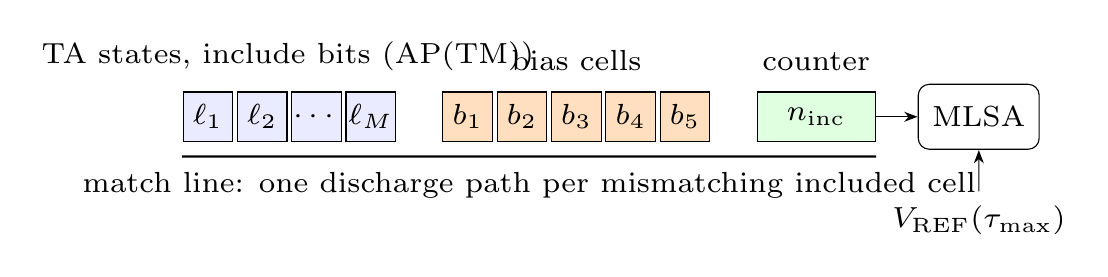
\begin{tikzpicture}[scale=1.5, transform shape, font=\scriptsize, cell/.style={draw, minimum width=0.42cm, minimum height=0.42cm, inner sep=0pt}, >=Stealth]
\foreach \i/\t in {0/$\ell_1$,1/$\ell_2$,2/$\cdots$,3/$\ell_M$} {\node[cell, fill=blue!8] (L\i) at (\i*0.46,0) {\t};}
\node[above=0.05cm of L1.north east, anchor=south] {TA states, include bits (AP(TM))};
\foreach \i/\t in {0/1,1/2,2/3,3/4,4/5} {\node[cell, fill=orange!25] (B\i) at (2.2+\i*0.46,0) {$b_{\t}$};}
\node[above=0.05cm of B2.north, anchor=south] {bias cells};
\node[cell, minimum width=1.0cm, fill=green!12] (N) at (5.15,0) {$n_{\mathrm{inc}}$};
\node[above=0.05cm of N.north, anchor=south] {counter};
\node[draw, rounded corners, minimum width=0.9cm, minimum height=0.55cm, right=0.35cm of N] (SA) {MLSA};
\draw[->] (N.east) -- (SA.west);
\node[below=0.35cm of SA] (REF) {$V_{\mathrm{REF}}(\tau_{\max})$};
\draw[->] (REF.north) -- (SA.south);
\draw[thick] ($(L0.south west)+(0,-0.12)$) -- ($(N.south east)+(0,-0.12)$) node[midway, below] {match line: one discharge path per mismatching included cell};
\end{tikzpicture}
\caption{AP(TM) row with the QM additions (shaded orange and green). Bias cell $b_t$, $t = 1, \dots, \tau_{\max}$, mismatches on every search if $\tau_j < t$, so the global threshold $\tau_{\max}$ yields the per-row tolerance $\tau_j$. Drawing not to scale.}
\label{fig:row}
\end{figure}

\subsection{QM clause evaluation}
Compare-tm discharges the match line through every included literal that is false, so the number of discharge paths is $v_j$.
A threshold compare-tm with reference $\tau$ therefore declares a match if $v_j \le \tau$.
With a threshold common to all rows, Eq.~\eqref{eq:qm} still needs a per-row tolerance $\tau_j$.
We add $\tau_{\max}$ bias cells per row.
Bias cell $b_t$, $t = 1, \dots, \tau_{\max}$, is written to mismatch on every search if $\tau_j < t$, and to match otherwise.
Row $j$ then has $v_j + (\tau_{\max} - \tau_j)$ mismatches, and the global threshold $\tau_{\max}$ gives
\begin{equation}
v_j + \tau_{\max} - \tau_j \le \tau_{\max} \iff v_j \le \tau_j .
\end{equation}
The bias cells must be refreshed when $\ninc$ changes, which happens only during training.

\textbf{Clamped tolerance.} Type~II feedback is not limited by the literal budget, so $\ninc$ and $\tau_j$ are not bounded.
The hardware therefore clamps the tolerance at $\tau_{\max} = 5$:
\begin{equation}
\tau_j^{\mathrm{hw}} = \min\left(\left\lfloor (1-\theta)\,\ninc \right\rfloor, \tau_{\max}\right).
\end{equation}
This equals Eq.~\eqref{eq:qm} for clauses with up to 59 ($\theta = 0.90$) or 119 ($\theta = 0.95$) included literals.
We inspected the largest clause every five epochs in the six cells where QM wins, for tuning seed~1 and test seed~101.
Its size ranged from 35 to 76 literals, within these limits, at all checkpoints but one: on UCI HAR with 5 clauses per class and $\theta = 0.90$, it held 60 literals at epoch~5 of seed~101, where the clamp gives a tolerance of 5 instead of 6.
The QM cells of the density-rule test (Section~\ref{sec:res-rule}) and the other test seeds were not inspected.
The accuracy results of Section~\ref{sec:results} were obtained with the unclamped rule of Eq.~\eqref{eq:qm}.
We did not re-run them with the clamp.

\add{\subsection{QP clause evaluation}
\label{sec:hw-qp}
Let $n_{\mathrm{pos},j}$ be the number of included positive literals of clause $j$, and $v_j^{+}$ the number of them that are false on the sample.
A QP clause fires if none of its included negated literals is false and $v_j^{+} \le \tau_j^{+} = \lfloor (1-\theta)\,n_{\mathrm{pos},j} \rfloor$.
The two conditions have different tolerances, so one threshold compare-tm cannot evaluate them together.
QP therefore uses two compare-tm operations with modified search keys.
A literal cell discharges the match line only if its literal is included and its search-line value is false.
Driving the search lines of a group of literals to true thus removes that group from the compare.
First, an exact compare-tm with the positive-literal columns driven true tags the rows whose included negated literals are all true.
One write stores this tag in a row flag $F_1$.
Second, a threshold compare-tm with the negated-literal columns driven true counts only $v_j^{+}$.
With the bias cells set from $\tau_j^{+}$ as in Section~\ref{sec:hw}, it tags the rows with $v_j^{+} \le \tau_j^{+}$.
One write stores this tag in a row flag $F_2$.
Third, an exact compare on $F_1 = F_2 = 1$ gives the clause outputs.
QP evaluation thus takes three compares and two writes instead of one compare, \proj{four additional cycles per evaluation}.
This is below \proj{0.02\,\%} of the cycles of Eq.~\eqref{eq:aptmcycles} for every encoding.

An arm uses either QM or QP, so QP reuses the $\tau_{\max} = 5$ bias cells of QM.
They are refreshed from $n_{\mathrm{pos},j}$ instead of $\ninc$.
For $\theta = 0.01$ and $0.10$, the clamped tolerance equals $\tau_j^{+}$ for clauses with up to six included positive literals.
A saturating counter of $c' = 3$ bits per row holds $n_{\mathrm{pos},j}$.
It is incremented in the recount pass of Section~\ref{sec:hw-count}, for the $M/2$ positive literals only, with the include tag and the increment enable of $\ninc$.
This adds $(4c'+3)\,M/2$ cycles per class update, and the bias refresh takes at most $\tau_{\max}(2c'+2) = 40$ cycles.
Over all encodings, QP with $L = 64$ adds \proj{49.4 to 53.1\,\%} to the training cycles of Eq.~\eqref{eq:aptmcycles}.
This is \proj{9.0 to 9.4} percentage points more than the literal budget alone.
The counter and the two flags widen the row by \proj{at most 1.33\,\%}.}

\subsection{Included-literal counter and literal budget}
\add{\label{sec:hw-count}}
The literal budget needs $\ninc \le L$ before each Type~I decision, and the bias cells need $\tau_j^{\mathrm{hw}}$.
Each row holds a saturating counter of $c$ bits that resolves $\ninc$ up to $\max(L+1, \lceil \tau_{\max}/(1-\theta) \rceil)$, so $c = 6$ or~7.
After the feedback phase of every class update, the controller recounts $\ninc$.
It clears the counters, and for each literal it tags the rows whose TA is in the include half and increments their counters with the saturating increment of AP(TM) (Algorithm~1 of~\cite{shrot2026aptm}, $2c+1$ compares and $2c+2$ writes).
This takes $(4c+5)M + 1$ cycles.
For $L = 2^k$, the budget test is two compares and one write per class update.
The extra Type~Ib branch for firing clauses over the budget adds one compare and one write per literal.
The bias refresh takes at most $\tau_{\max}(2c+2)$ cycles per class update.

\subsection{R1}
\maskred{AP(TM) sets the decrement enable of Type~Ib with a compare on the row's polarity, output and stochastic mask bit~\cite{shrot2026aptm}.}
R1 adds the literal's input bit, which is already on the search lines, to this compare.
It \proj{adds no cycle and one compared bit}.

\subsection{Projected cost}
\label{sec:hwcost}
Table~\ref{tab:hw} summarizes the \proj{projected} overhead.
Inference uses one threshold compare-tm in place of the exact one.
Its cycle count is \proj{unchanged} under the assumption below.
We assume that a threshold compare takes one cycle and the energy that AP(TM)~\cite{shrot2026aptm} assumes for an exact compare. The circuit-level cost of the programmable reference is not modeled.
Training is dominated by the recount, which grows with $M$ like the feedback phase itself.
It adds \proj{\numhwLmindc{} to \numhwLmaxge{}\,\%} of the cycles of Eq.~\eqref{eq:aptmcycles}, depending on $c$ and $s$.
These overheads are relative to AP(TM) as published, which has no literal budget.
The overhead is caused by the literal budget, which R1 and QM need\add{ (Section~\ref{sec:res-noL})}, and not by the QM threshold itself.
The vanilla TM selected on validation in our experiments also uses a literal budget in most cells (Section~\ref{sec:results}), so its AP(TM) mapping would need the same counter.
Against that baseline, R1 adds \proj{no training cycles} and QM adds only the bias refresh, \proj{at most 80 cycles per class update}.
An incremental update that detects include transitions during the feedback phase would avoid most of the recount when few transitions occur.
We did not evaluate it.

\begin{table*}[!htbp]
\centering
\caption{\proj{Projected} AP(TM) overhead of the additions, over all 26 encodings and $s \in \{2.5, 10\}$. Training cycles relative to Eq.~\eqref{eq:aptmcycles}. Row width relative to the AP(TM) row.}
\label{tab:hw}
\small
\begin{tabular}{lccc}
\toprule
Addition & Inference & Training cycles & Row width \\
\midrule
R1 & \proj{0 cycles} & \proj{0 cycles} & \proj{0 bits} \\
Literal budget ($c$-bit counter) & \proj{0 cycles} & \proj{+\numhwLmindc{} to +\numhwLmaxge{}\,\%} & \proj{+$c$ bits} \\
QM threshold and bias cells & \proj{0 cycles} & \proj{$\le$ 80 cycles} & \proj{+5 bits} \\
All \add{ but QP}, worst case & \proj{0 cycles} & \proj{+\numhwLmaxge{}\,\%} & \proj{$\le$ +\numhwareamax{}\,\%} \\
\add{QP with $L = 64$ (all its additions)} & \proj{+4 cycles} & \proj{+49.4 to +53.1\,\%} & \proj{$\le$ +1.33\,\%} \\
\bottomrule
\end{tabular}
\end{table*}

The area and energy of AP(TM) scale with the number of rows, $C \cdot K$~\cite{shrot2026aptm}.
A configuration that reaches the accuracy of the vanilla TM with fewer clauses per class therefore \proj{saves array area and search energy in proportion}.
Section~\ref{sec:res-budget} measures this ratio.

%% ---------------------------------------------------------------------------
\section{Experimental setup}
\label{sec:setup}

\subsection{Datasets and encodings}
Table~\ref{tab:datasets} lists the datasets.
MNIST~\cite{lecun1998mnist}, Fashion-MNIST~\cite{xiao2017fmnist}, UCI Adult~\cite{kohavi1996adult} and IMDb~\cite{maas2011imdb} use the Boolean encodings of AP(TM)~\cite{shrot2026aptm}.
UCI HAR~\cite{anguita2013har} uses ten thresholds per feature at the training quantiles 5 to \SI{95}{\percent}, and UCI Phishing~\cite{mohammad2014phishing} one-hot codes its categorical features.
The text sets are R8 and R52~\cite{cardoso2007r8}, 20 Newsgroups~\cite{lang1995newsweeder}, Sector~\cite{rennie2001sector}, RCV1~\cite{lewis2004rcv1} and LEDGAR~\cite{tuggener2020ledgar,chalkidis2022lexglue}.
Dorothea~\cite{guyon2004dorothea} is a sparse binary drug-discovery set with 100,000 features.
R8, R52 and LEDGAR are encoded from raw text as a binary bag of words: lowercase alphabetic tokens of two or more characters, NLTK English stop words~\cite{bird2009nltk} removed, and document frequency of at least two.
Sector, 20 Newsgroups and RCV1 come from the LIBSVM collection~\cite{chang2011libsvm}, and their features are binarized as presence indicators.
For all text sets and Dorothea, chi-square selection of $V$ features uses the training part only.
Several sets appear at several vocabulary sizes $V$, so that density varies within a dataset.
Validation data are the official split if one exists, otherwise a stratified \SI{10}{\percent} of the training split (\SI{15}{\percent} for R8, R52 and Dorothea).
The official Dorothea validation set serves as its test set, and the UCI Phishing test set is a stratified \SI{20}{\percent} split.
The RCV1 test set is a random sample of 50,000 documents of the official test file.
The six datasets marked $\dagger$ were added after study~1 to test the density rule (Section~\ref{sec:res-rule}): AG News~\cite{zhang2015agnews}, TREC-6~\cite{li2002trec}, Emotion~\cite{saravia2018emotion}, USPS~\cite{hull1994usps}, Letter~\cite{frey1991letter} and Satimage~\cite{michie1994statlog}.
The three added text sets use the raw-text encoding above. TREC-6 keeps stop words, because its classes are defined by question words. \hadd{Letter, USPS and Satimage come from the LIBSVM collection~\cite{chang2011libsvm} and use ten thresholds per feature at the training quantiles 5 to 95\,\%, as UCI HAR.}

\begin{table*}[!htbp]
\centering
\caption{Datasets and encodings, ordered by training-set density. Active: mean number of true input bits per sample. $C$: clause budgets per class tested. $\dagger$: added for the out-of-sample density rule.}
\label{tab:datasets}
\footnotesize
\setlength{\tabcolsep}{5pt}
\input{tab_datasets}
\end{table*}

\subsection{Protocol}
\label{sec:protocol}
The evaluation has three parts. Study~1 (Section~\ref{sec:res-main}) compares all arms on 20 encodings. Study~2 tests a density rule on six new datasets (Section~\ref{sec:res-rule}) and sweeps the clause budget (Section~\ref{sec:res-budget}). The baseline controls (Section~\ref{sec:res-base}) strengthen the vanilla TM. They were designed after all Study~1 and Study~2 results were known, in response to a review, and their protocol was written before their runs.
\add{A symmetric control and a literal-budget ablation (Sections~\ref{sec:res-base} and~\ref{sec:res-noL}) were designed after the baseline controls, in response to a second review. Their protocol was also written before their runs.}
Each protocol was written before its runs and amended only before the affected runs. The protocols are internal documents, not external registrations, and are released with the code and all logs.
The two amendments of Study~1 added datasets, reduced the grid for them, and excluded three encodings for run time and memory.
The Study~1 protocol specifies a \SI{10}{\percent} validation split. The R8, R52 and Dorothea encodings, prepared earlier, use \SI{15}{\percent}.
The Study~2 protocol also specified a comparison with the reference code of the Fuzzy-Pattern TM~\cite{hnilov2025fptm}. It was run but is not reported, because that work is not peer reviewed and its graded vote does not map to one threshold search (Section~\ref{sec:related}).
Clause budgets are $C = 5, 10, 20$ per class with $T = 3, 5, 10$ for the eight original encodings, and $C = 5, 10$ for the twelve added ones.
Specificity $s$ is tuned per arm over $\{2.5, 5, 10\}$, or $\{2.5, 10\}$ for the added encodings.
All runs train for 40 epochs.
For each dataset, budget and arm, the configuration and $s$ with the highest validation accuracy at the last epoch on tuning seed~1 are selected (ties: smaller $s$, then the first listed configuration).
The selected settings are then trained with seeds 101 to 105 and evaluated once on the test split.
The best QM-family arm and the best non-QM arm of each cell are also chosen on validation.

\textbf{Baseline controls.} In Study~1 the vanilla TM selected $s = 2.5$, the smallest grid value, in 42 of 48 cells, and its family lacked the budget $L = 32$ that TMR and QM use.
The controls therefore define an extended vanilla family, TM$_{\mathrm{ext}}$: no budget, $L = 64$ and $L = 32$, each with the original $s$ grid plus $s = 1.5$.
TM$_{\mathrm{ext}}$ is selected with the rule above on all 48 Study~1 and 12 Study~2 cells, reusing the original vanilla runs, and confirmed with seeds 101 to 105 where its selection changes.
Every contrast is then recomputed against TM$_{\mathrm{ext}}$.
Only the vanilla TM is strengthened: the modified arms keep their original grid, selections and test runs.
\add{The symmetric control then adds $s = 1.5$ to the grid of TMR, QM and QMR in each cell.
These arms are re-selected with the same rule, reusing their original runs, and confirmed with seeds 101 to 105 where the selection changes.
QP and QPR are not re-tuned.
The symmetric control covers the 48 Study~1 and the 12 Study~2 cells.}
\add{The literal-budget ablation removes $L$ from the TMR and QM settings selected in the symmetric control, keeps $s$ and $T$, and runs seeds 101 to 103.
An arm counts as working without the budget only if it has no significant loss against the budgeted arm, its median difference exceeds $-1$~pp, and it is within 1~pp in at least three quarters of the cells.
This criterion was fixed before the runs.}
The controls can only raise the validation accuracy of the baseline. On test data it fell in 7 of 60 cells, by at most 1.3~pp.
In the budget sweep, the vanilla TM is re-tuned at each budget from 40 to 160 clauses per class over $\{L = 32, L = 64\} \times \{1.5, 2.5\}$ and its original setting, and confirmed with seeds 101 to 103.
\add{In the symmetric control, TMR and QM are re-tuned in the same way at each budget from 40 to 160 clauses per class, over their original sweep setting and every member of their family at {$s = 1.5$}, with seed~1 on validation. A changed selection is confirmed with seeds 101 to 103. IMDb is not included.}
\hnote{Why is IMDb excluded from the symmetric control and the re-tuned sweep?}

\subsection{Statistics}
The unit of analysis is the seed. Accuracy differences are given in percentage points (pp).
Each contrast compares the five test accuracies of two arms with Welch's $t$-test~\cite{welch1947}.
Holm's procedure~\cite{holm1979} controls the family-wise error at 0.05 within each contrast over the 48 cells.
The protocol fixed six contrasts: TMR$-$TM, QM$-$TM, QP$-$TM, QMR$-$TMR, QPR$-$TMR, and best QM-family arm minus best non-QM arm.
The split of cells at \SI{3}{\percent} density was chosen after Study~1. Any threshold between 2.1 and \SI{13.5}{\percent} separates the Study~1 encodings identically.
The relation of gain to input density and to the number of active features per sample is descriptive (Spearman correlation over cells, which are not independent within a dataset).

\subsection{Implementation}
All arms use pyTsetlinMachine~0.6.6~\cite{pytsetlinmachine}, patched for QM, QP and R1.
\maskred{With $\theta = 1$, standard feedback and the original feedback sampler, the patched code reproduces the original bit for bit, in predictions and in all TA states.
For speed, all runs, including the vanilla TM, select the literals that receive feedback with an independent Bernoulli($1/s$) mask per literal instead of the original sampled-count scheme. The marginal selection probability is the same, but the random stream differs.}
Inputs are packed into 32-bit words once per run.
The patches, the experiment scripts and the analysis code were written with Claude (Anthropic), a generative AI assistant, under the direction of the authors.
Study~1 comprised 1,560 tuning runs and 1,440 test runs, and the baseline controls \ctlTuneRuns{} tuning runs and \ctlTestRuns{} test runs\add{, and the symmetric control, the ablation and the sweep with re-tuned TMR and QM \fiveTuneRuns{} tuning runs and \fiveTestRuns{} test runs}, all on two CPU cores.

%% ---------------------------------------------------------------------------
\section{Results}
\label{sec:results}

\subsection{R1 and QM against the vanilla TM}
\label{sec:res-main}
This section and the next report the contrasts against the vanilla TM as tuned in the Study~1 protocol. Section~\ref{sec:res-base} repeats them against a stronger vanilla TM.
Table~\ref{tab:contrasts} summarizes the six contrasts, and Fig.~\ref{fig:density} plots the gains against input density.
The per-cell results are in Table~\ref{tab:study1} (\ref{app:cells}).

\begin{table}[!htbp]
\centering
\caption{Study~1 contrasts over 48 cells against the original vanilla TM (test accuracy, five seeds, Welch, Holm). Sparse: training density below \SI{3}{\percent} (\numnsparse{} cells). Dense: the other \numndense{}.}
\label{tab:contrasts}
\footnotesize
\setlength{\tabcolsep}{5pt}
\begin{tabular}{lccccc}
\toprule
Contrast & Wins & Losses & \multicolumn{2}{c}{Median gain (pp)} & Spearman \\
 & & & sparse & dense & $\rho$ (density) \\
\midrule
TMR $-$ TM & \numRwin & \numRloss & \numRmedsparse & \numRmeddense & \numRrho \\
QM $-$ TM & \numQwin & \numQloss & \numQmedsparse & \numQmeddense & \numQrho \\
QP $-$ TM & \numPwin & \numPloss & \numPmedsparse & \numPmeddense & \numPrho \\
QMR $-$ TMR & \numQRwin & \numQRloss & \numQRmedsparse & \numQRmeddense & \numQRrho \\
QPR $-$ TMR & \numPRwin & \numPRloss & \numPRmedsparse & \numPRmeddense & \numPRrho \\
Best QM $-$ best other & \numBwin & \numBloss & \numBmedsparse & \numBmeddense & \numBrho \\
\bottomrule
\end{tabular}
\end{table}

\begin{figure}[!htbp]
\centering
\includegraphics[width=0.6\textwidth]{figures/fig_density.pdf}
\caption{Test accuracy gain per (dataset, budget) cell against training-set input density. Circles: R1 (TMR $-$ TM). Squares: QM (best QM-family arm $-$ best non-QM arm). Filled markers: significant after Holm correction. Open markers: not significant. Dashed line: the \SI{3}{\percent} density boundary of the rule in Section~\ref{sec:res-rule}.}
\label{fig:density}
\end{figure}

\textbf{R1.} R1 is the larger effect.
It is significantly better than the vanilla TM in \numRwin{} cells and worse in \numRloss{}.
All significant gains are on sparse inputs, where the median gain is \numRmedsparse{}~pp and \numRpossparse{} of \numnsparse{} cells are positive.
The largest gains occur on Sector, 20 Newsgroups and RCV1, which combine many classes with very sparse inputs: +22.6 and +23.6~pp on Sector with 10 clauses per class.
All significant losses are on dense or one-hot inputs: MNIST and Fashion-MNIST at 10 and 20 clauses, and UCI Phishing, where R1 loses about 20~pp.
The gain falls with density (Spearman $\rho = $ \numRrho{}, $p = \numRrhop$). It is not correlated with the number of active features per sample ($\rho = -0.06$, $p = 0.71$).

\textbf{QM.} QM is a smaller, dense-input effect.
The best QM-family arm is significantly better than the best non-QM arm in \numBwin{} cells and worse in none.
All six are dense: MNIST at 10 clauses (+1.23~pp), Fashion-MNIST at 5, 10 and 20 (+2.93, +3.28, +3.84~pp) and HAR at 5 and 10 (+5.33 and +3.90~pp, with R1).
On sparse inputs the best QM arm is not significantly different from the best non-QM arm: median \numBmedsparse{}~pp, 17 of 35 cells positive, no significant difference.
The QM$-$TM gain is weakly correlated with density ($\rho = $ \numQrho{}, $p = 0.10$) and more strongly with the number of active features per sample ($\rho = 0.37$, $p = 0.01$).
QM with R1 recovers much of the loss that R1 causes on dense inputs (QMR$-$TMR, median \numQRmeddense{}~pp on dense cells) but loses to TMR on sparse ones (median \numQRmedsparse{}~pp).

\textbf{Negative results.} The polarity-aware variant does not help.
QP and QPR have no significant win against their baselines and two significant losses each.
At the validation stage, QPR appeared 1.1 to 5.4~pp better than TMR in 10 of the 15 R52 and 20 Newsgroups cells, and worse in 4.
This did not replicate on fresh seeds (QPR$-$TMR median on sparse cells \numPRmedsparse{}~pp), which illustrates the optimism of selecting the best member of an arm on one validation seed.

\subsection{Out-of-sample density rule}
\label{sec:res-rule}
Study~1 suggests a simple rule: use R1 if the training density is below \SI{3}{\percent} and QM otherwise.
We fixed this rule and the six new datasets of Table~\ref{tab:datasets} before running them.
The hypothesis fixed in advance is that the arm chosen by the rule beats the vanilla TM.
The rule counts as confirmed if it has more significant wins than losses and no significant loss.
Table~\ref{tab:rule} gives the results for $C = 5$ and 10.

\begin{table}[!htbp]
\centering
\caption{Out-of-sample density rule on six datasets not used in study~1 (test accuracy, mean of five seeds). Rule: R1 (TMR) below \SI{3}{\percent} density, QM otherwise. $\Delta$ rule: rule arm minus TM. $\Delta$ other: the other family minus TM, for reference. Bold: significant after Holm correction over the 12 cells of the respective contrast.}
\label{tab:rule}
\footnotesize
\setlength{\tabcolsep}{5pt}
\input{tab_rule}
\end{table}

Against the original vanilla TM, the rule is confirmed.
The rule arm is significantly better than the vanilla TM in \numruleWin{} of \numruleN{} cells and never significantly worse.
It is ahead in \numrulePos{} of \numruleN{} cells (one-sided sign test, $p = \numruleSignP$).
R1 gains 27.6 and 23.1~pp on AG News with 5 and 10 clauses.
QM gains 4.7 and 3.5~pp on USPS and 1.7~pp on Satimage with 10 clauses.
On Emotion and TREC-6, the rule arm is not significantly different from TM.
On these two small sets, both arms vary widely across seeds, with standard deviations of 7.0 to 12.0~pp for R1 and 0.8 to 8.8~pp for the vanilla TM.

The rule also matters.
Applying the other family instead gives \numotherWin{} significant win and \numotherLoss{} significant losses.
QM on the three sparse sets loses 5.8 to 16.0~pp, three times significantly.
In study~1, QM had no significant loss in any cell, but the sparsest study~1 encoding has \SI{0.34}{\percent} density. The three new text sets, at 0.11 to \SI{0.28}{\percent}, show that QM can hurt very sparse inputs, which supports routing them to R1.
R1 on the dense sets is closer to neutral here than in study~1, and it is significantly better than TM on USPS with 5 clauses.
Against the stronger baseline of Section~\ref{sec:res-base}, the rule is not confirmed.

\subsection{Baseline controls}
\label{sec:res-base}
Table~\ref{tab:controls} repeats the contrasts of Sections~\ref{sec:res-main} and~\ref{sec:res-rule} against the extended vanilla family TM$_{\mathrm{ext}}$ (Section~\ref{sec:setup}).
The selection of the vanilla TM changed in \ctlChangedOne{} of \ctlCellsOne{} Study~1 cells and in all \ctlCellsTwo{} Study~2 cells.
TM$_{\mathrm{ext}}$ chose $s = 1.5$ in \ctlSlowOne{} and \ctlSlowTwo{} of these cells, and $L = 32$ in \ctlLthreeOne{} and \ctlLthreeTwo{}.
Its test accuracy exceeds that of the original vanilla TM by a median of 1.7~pp in Study~1 (2.0~pp on sparse and 0.6~pp on dense cells) and 3.6~pp in Study~2.
The largest increases are 15.0~pp on Sector with 20,000 words and 10 clauses per class, and 28.3~pp on AG News with 5.
Because $s = 1.5$ is the smallest value tried, the vanilla TM may not be fully tuned even now.

\begin{table*}[!htbp]
\centering
\caption{Contrasts against the original vanilla TM and against the extended vanilla family TM$_{\mathrm{ext}}$ (test accuracy, five seeds, Welch, Holm within each contrast and baseline). W/L: significant wins and losses. Med.: median gain in pp. Sparse: training density below \SI{3}{\percent}. \del{Only the vanilla TM is re-tuned.} \add{Original: neither arm re-tuned. Extended: only the vanilla TM re-tuned. Both re-tuned: $s = 1.5$ also offered to TMR, QM and QMR. QP and QPR are not re-tuned.} ``Best other'' is the better of TMR and the vanilla TM on validation. The Study~2 TMR and QM rows are descriptive additions to the control protocol.}
\label{tab:controls}
\vspace{3pt}
\small
\begin{tabular}{llcccccc}
\toprule
 & & \multicolumn{2}{c}{All cells} & \multicolumn{2}{c}{Sparse} & \multicolumn{2}{c}{Dense} \\
\cmidrule(lr){3-4}\cmidrule(lr){5-6}\cmidrule(lr){7-8}
Contrast & Baseline & W/L & Med. & W/L & Med. & W/L & Med. \\
\midrule
\multicolumn{8}{l}{\emph{Study~1, 48 cells}} \\
TMR $-$ TM & original & 24/6 & +2.60 & 24/0 & +6.26 & 0/6 & $-$4.37 \\
 & extended & 10/7 & +0.15 & 10/1 & +1.32 & 0/6 & $-$5.43 \\
 & {\color{blue}both re-tuned} & {\color{blue}19/8} & {\color{blue}+1.61} & {\color{blue}19/0} & {\color{blue}+3.67} & {\color{blue}0/8} & {\color{blue}$-$5.43} \\
QM $-$ TM & original & 5/0 & $-$0.11 & 0/0 & $-$0.83 & 5/0 & +1.23 \\
 & extended & 4/13 & $-$2.67 & 0/12 & $-$4.23 & 4/1 & +0.62 \\
 & {\color{blue}both re-tuned} & {\color{blue}8/2} & {\color{blue}$-$0.57} & {\color{blue}4/2} & {\color{blue}$-$1.32} & {\color{blue}4/0} & {\color{blue}+0.95} \\
QP $-$ TM & original & 0/2 & +0.13 & 0/0 & +0.45 & 0/2 & $-$0.52 \\
 & extended & 0/15 & $-$1.25 & 0/11 & $-$1.15 & 0/4 & $-$1.89 \\
Best QM $-$ best other & original & 6/0 & +0.06 & 0/0 & $-$0.04 & 6/0 & +1.05 \\
 & extended & 6/2 & $-$0.02 & 0/0 & $-$0.04 & 6/2 & +1.23 \\
 & {\color{blue}both re-tuned} & {\color{blue}4/1} & {\color{blue}$-$0.64} & {\color{blue}0/1} & {\color{blue}$-$1.58} & {\color{blue}4/0} & {\color{blue}+0.95} \\
\midrule
\multicolumn{8}{l}{\emph{Study~2, six new datasets, 12 cells}} \\
Rule arm $-$ TM & original & 5/0 & +2.59 & 2/0 & +7.36 & 3/0 & +1.55 \\
 & extended & 2/3 & $-$0.04 & 0/2 & $-$2.47 & 2/1 & +0.77 \\
 & {\color{blue}both re-tuned} & {\color{blue}3/2} & {\color{blue}+0.85} & {\color{blue}2/1} & {\color{blue}+8.52} & {\color{blue}1/1} & {\color{blue}+0.17} \\
TMR $-$ TM & original & 3/0 & +0.89 & 2/0 & +7.36 & 1/0 & +0.40 \\
 & extended & 0/4 & $-$1.26 & 0/2 & $-$2.47 & 0/2 & $-$1.26 \\
 & {\color{blue}both re-tuned} & {\color{blue}2/3} & {\color{blue}$-$0.67} & {\color{blue}2/1} & {\color{blue}+8.52} & {\color{blue}0/2} & {\color{blue}$-$1.26} \\
QM $-$ TM & original & 3/3 & $-$2.53 & 0/3 & $-$13.59 & 3/0 & +1.55 \\
 & extended & 2/6 & $-$6.15 & 0/5 & $-$22.73 & 2/1 & +0.77 \\
 & {\color{blue}both re-tuned} & {\color{blue}1/6} & {\color{blue}$-$6.08} & {\color{blue}0/5} & {\color{blue}$-$18.64} & {\color{blue}1/1} & {\color{blue}+0.17} \\
\bottomrule
\end{tabular}

\end{table*}

\textbf{R1.} Against TM$_{\mathrm{ext}}$, R1 wins \ctlRextallW{} Study~1 cells and loses \ctlRextallL{}.
All wins are on sparse many-class text: RCV1 (+11.7 and +10.0~pp), Sector (+7.6 and +8.5~pp), R52 (+3.0 to +5.5~pp) and R8 (+3.3~pp).
On sparse cells R1 still wins \ctlRextsparseW{} times and loses once, on 20 Newsgroups with 1,000 words and 5 clauses per class, but its median gain falls from \ctlRorigsparseMed{} to \ctlRextsparseMed{}~pp.
It still loses on dense cells, by up to 23.4~pp on UCI Phishing.
In Study~2, R1 has no significant win against TM$_{\mathrm{ext}}$ and loses \ctlSRextallL{} cells, all with 10 clauses per class: AG News (4.3~pp), TREC-6 (15.4~pp), Letter (5.3~pp) and USPS (1.7~pp).
Tuning the vanilla TM recovers most of the original R1 gain on these sets: on AG News the vanilla TM itself gains 28.3 and 27.4~pp from the extended grid.
\add{With $s = 1.5$ offered to R1 as well, R1 wins \ctlRbothallW{} Study~1 cells against TM$_{\mathrm{ext}}$ and loses \ctlRbothallL{}.
All wins are on sparse text, by 1.5 to 17.2~pp: Sector, RCV1, 20 Newsgroups, R52, R8, LEDGAR and IMDb (1.5~pp with 20 clauses per class).
All losses are on dense cells: MNIST and Fashion-MNIST at all three budgets (4.2 to 7.7~pp) and UCI Phishing (18.1 and 19.4~pp).
R1 selected $s = 1.5$ in \selFiveROneSlow{} of \selFiveROneN{} cells. Offering it raised the accuracy of R1 significantly in \ctlRselfSW{} cells and lowered it in none (median \ctlRselfSMed{}~pp).
In Study~2, R1 with $s = 1.5$ wins on Emotion (+19.8 and +25.0~pp) and loses on Letter, AG News and USPS with 10 clauses (5.3, 2.2 and 1.7~pp).}

\textbf{QM.} Plain QM loses to TM$_{\mathrm{ext}}$ in \ctlQextallL{} Study~1 cells and wins \ctlQextallW{}.
All losses but one are on sparse text, where QM had no significant loss against the original baseline.
On dense cells QM wins \ctlQextdenseW{} times (Fashion-MNIST at 5, 10 and 20 clauses and MNIST at 10, by 1.2 to 3.5~pp) and loses once (UCI Phishing at 10 clauses, 2.3~pp).
The best QM-family arm against the better of TM$_{\mathrm{ext}}$ and TMR wins \ctlBextdenseW{} dense cells and loses \ctlBextdenseL{}: it adds QMR on UCI HAR (+5.5 and +2.4~pp) and loses on UCI Phishing with 10 clauses (2.3~pp) and UCI Adult with 20 (0.4~pp).
In Study~2, QM beats TM$_{\mathrm{ext}}$ on USPS (+1.7 and +1.0~pp). On the dense sets it loses only on Letter with 10 clauses (2.9~pp), and it loses \ctlSQextsparseL{} cells on the three text sets.
QP loses \ctlPextallL{} cells and wins none.
\add{With $s = 1.5$ offered to QM as well, QM wins \ctlQbothallW{} Study~1 cells and loses \ctlQbothallL{}.
It wins on Fashion-MNIST at all three budgets and on MNIST at 10 clauses (1.2 to 3.5~pp), and on Sector with 5,000 and 20,000 words (6.8 to 10.9~pp).
It loses on Sector with 1,000 words (6.5~pp) and on R52 with 1,000 words and 20 clauses (3.6~pp).
Offering $s = 1.5$ raised the accuracy of QM significantly in \ctlQselfSW{} cells, all but one on Sector and 20 Newsgroups, and lowered it in none.
The best QM-family arm wins \ctlBbothallW{} cells, on MNIST and Fashion-MNIST, and loses \ctlBbothallL{}, on 20 Newsgroups with 1,000 words (5.7~pp).
In Study~2, QM with $s = 1.5$ wins only on USPS with 10 clauses (1.0~pp). It loses \ctlSQbothallL{} cells: five on the three text sets (16.2 to 23.1~pp) and Letter with 10 clauses (2.8~pp).}

\textbf{Density rule.} As a descriptive check outside the control protocol, the rule applied to Study~1, where it was derived, beats TM$_{\mathrm{ext}}$ in \ctlSoneRuleW{} cells and loses in \ctlSoneRuleL{}, with significance taken from the Holm-corrected TMR and QM contrasts.
On the six unseen datasets of Study~2, it wins \ctlruleextallW{} cells and loses \ctlruleextallL{}, and it is ahead in \ctlrulePos{} of 12 (one-sided sign test, $p = \ctlruleSignP$).
By the criterion fixed in Section~\ref{sec:res-rule}, the rule is not confirmed against the stronger baseline.
\add{With both arms re-tuned, the rule applied to Study~1 wins \ctlSoneRuleBothW{} of \ctlSoneRuleBothN{} cells and loses none.
On the six unseen datasets it wins \ctlrulebothallW{} cells (Emotion with 5 and 10 clauses, +19.8 and +25.0~pp, and USPS with 10, +1.0~pp) and loses \ctlrulebothallL{} (Letter and AG News with 10 clauses, 2.8 and 2.2~pp).
It is ahead in \ctlruleBothPos{} of 12 cells (one-sided sign test, $p = \ctlruleBothSignP$).
By the same criterion, the rule is again not confirmed.}

\textbf{Caveat.} The controls favor the baseline by design.
\del{The modified arms also selected the smallest $s$ in most cells (TMR in 42, QM in 30 of 48), so they might also gain from {$s = 1.5$}.}
\del{We did not run this symmetric control.}
\del{The results above therefore bound what the modifications add over a vanilla TM tuned on a finer grid, under tuning budgets that are not equal.}
\add{The symmetric control gives all arms the same $s$ grid.
TM$_{\mathrm{ext}}$ can also choose no literal budget, which TMR and QM cannot. Section~\ref{sec:res-noL} shows that this option lowers their accuracy.
TMR, QM and QMR selected $s = 1.5$, the smallest value offered, in \selFiveROneSlow{}, \selFiveQOneSlow{} and \selFiveQROneSlow{} of \selFiveROneN{} Study~1 cells.}

\add{\subsection{Literal-budget ablation}
\label{sec:res-noL}
The ablation tests whether R1 and QM need the literal budget $L$.
It removes $L$ from the TMR and QM settings of the symmetric control and keeps $s$ and $T$ (Section~\ref{sec:protocol}).
Table~\ref{tab:noL} compares the test accuracy with and without $L$ on the same seeds.}

\begin{table}[!htbp]
\centering
\add{\caption{Literal-budget ablation (test accuracy, seeds 101 to 103, Welch, Holm within each row). No budget $-$ budget: the same arm and setting without and with $L$. W/L: significant wins and losses. Med.: median difference in pp. Within 1~pp: cells with an absolute difference of at most 1~pp. Literals per clause: median over cells of the mean number of included literals per clause after training. Study~1: 48 cells. Study~2: 12 cells.}
\label{tab:noL}}
\footnotesize
\setlength{\tabcolsep}{5pt}
\add{\begin{tabular}{llcccccc}
\toprule
 & & \multicolumn{4}{c}{No budget $-$ budget} & \multicolumn{2}{c}{Literals per clause} \\
\cmidrule(lr){3-6}\cmidrule(lr){7-8}
Study & Arm & Cells & W/L & Med. & Within 1~pp & Budget & No budget \\
\midrule
1 & TMR & 45 & 0/36 & $-$40.50 & 2 & 50.9 & 4349.6 \\
1 & QM & 45 & 0/28 & $-$31.69 & 3 & 28.4 & 2542.2 \\
2 & TMR & 12 & 0/10 & $-$45.11 & 0 & 65.7 & 1900.3 \\
2 & QM & 12 & 0/4 & $-$7.41 & 1 & 23.1 & 1259.9 \\
\bottomrule
\end{tabular}
}
\end{table}

\add{Neither arm works without the budget.
Without $L$, R1 loses significantly in \noLROneL{} of \noLROneN{} Study~1 cells and \noLRTwoL{} of \noLRTwoN{} Study~2 cells, with median losses of 37.8 and 45.1~pp.
QM loses in \noLQOneL{} and \noLQTwoL{} cells, with median losses of 31.8 and 7.4~pp.
Neither arm wins a cell.
The median number of included literals per clause rises from 23 to 66 with the budget to 1,260 to 3,790 without it.
On UCI Phishing, where the clauses stay below the budget, removing $L$ changes the test accuracy by at most 0.14~pp.
Against TM$_{\mathrm{ext}}$, R1 without $L$ loses \noLROneTmL{} Study~1 and \noLRTwoTmL{} Study~2 cells, and QM without $L$ loses \noLQOneTmL{} and \noLQTwoTmL{}.
Both rules weaken the pressure that removes literals from a clause.
R1 no longer forgets the satisfied literals of a non-firing clause.
QM lets a clause fire with violated literals, so the clause receives Type~Ia instead of Type~Ib feedback.
The literal budget therefore limits clause growth for both rules, and its counter (Section~\ref{sec:hw-count}) is a necessary part of their hardware cost.}

\subsection{Clauses saved at equal accuracy}
\label{sec:res-budget}
The budget sweep extends the eight encodings tested at $C = 5$, 10 and 20 to $C = 40$, 80 and 160.
TMR and QM keep the configuration and $s$ selected at $C = 20$ in Study~1, with $T = C/2$, and run with seeds 101 to 103.
\add{The sweep also has re-tuned TMR and QM. They use the selection of the symmetric control at $C \le 20$ (Section~\ref{sec:res-base}) and are re-tuned at each larger budget (Section~\ref{sec:protocol}). The selection changed in \sweepFiveChanged{} of \sweepFiveN{} arm and budget pairs, 15 for TMR and 6 for QM, and every changed selection uses $s = 1.5$.}
The sweep has two vanilla baselines.
The original TM keeps its $C = 20$ setting, as the modified arms do.
The re-tuned TM uses TM$_{\mathrm{ext}}$ (Section~\ref{sec:res-base}) at $C \le 20$ and is re-tuned at each larger budget (Section~\ref{sec:protocol}).
The sweep is descriptive: it has no hypothesis test.
Fig.~\ref{fig:sweep} plots the mean test accuracy against $C$.
Table~\ref{tab:budget} gives, for the arm chosen by the density rule at $C = 5$ and 10, the smallest vanilla budget whose mean accuracy is at least as high.

\begin{figure*}[!htbp]
\centering
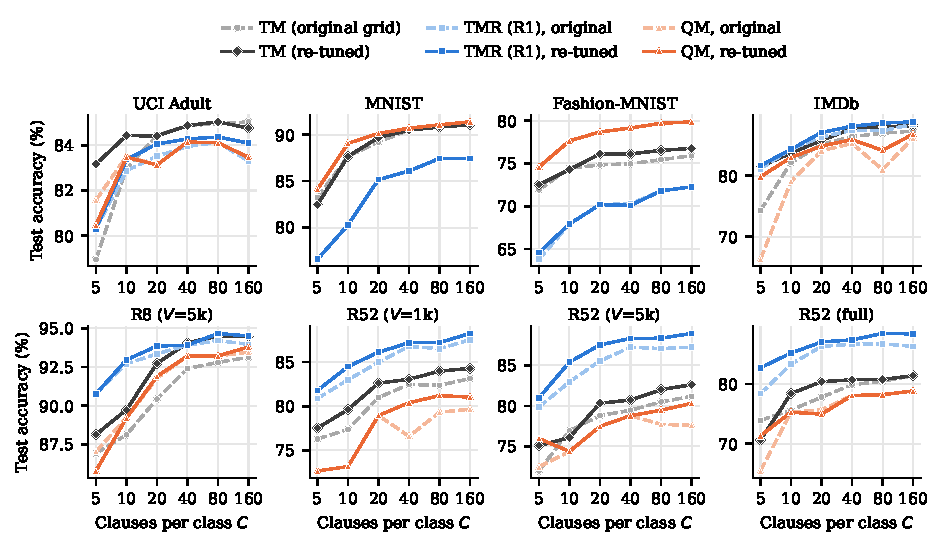
\includegraphics[width=\textwidth]{figures/fig_sweep.pdf}
\caption{Clause-budget sweep: mean test accuracy over seeds 101 to 103 against clauses per class $C$ (log scale). TMR, QM and the original TM: Study~1 settings at $C \le 20$, the $C = 20$ setting with $T = C/2$ at $C \ge 40$. Re-tuned TM: TM$_{\mathrm{ext}}$ at $C \le 20$, re-tuned per budget at $C \ge 40$. \add{Dashed TMR and QM: original settings. Solid TMR and QM: re-tuned, with the selection of the symmetric control at $C \le 20$ and re-tuned per budget at $C \ge 40$. IMDb has no re-tuned TMR or QM. Where the re-tuned selection equals the original one, the solid curve covers the dashed one.}}
\label{fig:sweep}
\end{figure*}

\begin{table}[!htbp]
\centering
\caption{Smallest vanilla clause budget per class (TM $C$ needed) whose mean test accuracy reaches that of the rule arm with 5 or 10 clauses per class. Orig.: original TM. Re-t.: re-tuned TM. Mean of seeds 101 to 103. $>$160: not reached in the sweep. \add{Second line (blue): the rule arm re-tuned in the symmetric control (Section~\ref{sec:res-base}). IMDb has no re-tuned rule arm.}}
\label{tab:budget}
\footnotesize
\setlength{\tabcolsep}{5pt}
\begin{tabular}{lrcrrrrrr}
\toprule
 & Dens. & Rule & \multicolumn{3}{c}{Rule arm, $C = 5$} & \multicolumn{3}{c}{Rule arm, $C = 10$} \\
\cmidrule(lr){4-6}\cmidrule(lr){7-9}
 & & & & \multicolumn{2}{c}{TM $C$ needed} & & \multicolumn{2}{c}{TM $C$ needed} \\
\cmidrule(lr){5-6}\cmidrule(lr){8-9}
Dataset & (\%) & arm & Acc. & orig. & re-t. & Acc. & orig. & re-t. \\
\midrule
R52 (full) & 0.38 & R1 & 78.41 & 40 & 10 & 83.34 & $>$160 & $>$160 \\
{\color{blue}\quad re-tuned} &  &  & {\color{blue}82.76} & {\color{blue}$>$160} & {\color{blue}$>$160} & {\color{blue}85.22} & {\color{blue}$>$160} & {\color{blue}$>$160} \\
R8 ($V$=5k) & 0.67 & R1 & 90.76 & 40 & 20 & 92.71 & 80 & 20 \\
{\color{blue}\quad re-tuned} &  &  & {\color{blue}90.76} & {\color{blue}40} & {\color{blue}20} & {\color{blue}92.96} & {\color{blue}160} & {\color{blue}40} \\
R52 ($V$=5k) & 0.68 & R1 & 79.85 & 80 & 20 & 82.96 & $>$160 & $>$160 \\
{\color{blue}\quad re-tuned} &  &  & {\color{blue}80.99} & {\color{blue}160} & {\color{blue}80} & {\color{blue}85.42} & {\color{blue}$>$160} & {\color{blue}$>$160} \\
R52 ($V$=1k) & 1.35 & R1 & 80.87 & 20 & 20 & 82.99 & 160 & 40 \\
{\color{blue}\quad re-tuned} &  &  & {\color{blue}81.80} & {\color{blue}40} & {\color{blue}20} & {\color{blue}84.49} & {\color{blue}$>$160} & {\color{blue}$>$160} \\
IMDb & 2.10 & R1 & 81.14 & 10 & 5 & 84.34 & 20 & 20 \\
{\color{blue}\quad re-tuned} &  &  & {\color{blue}81.67} & {\color{blue}10} & {\color{blue}10} & {\color{blue}84.34} & {\color{blue}20} & {\color{blue}20} \\
UCI Adult & 13.49 & QM & 81.57 & 10 & 5 & 83.51 & 20 & 10 \\
{\color{blue}\quad re-tuned} &  &  & {\color{blue}80.47} & {\color{blue}10} & {\color{blue}5} & {\color{blue}83.48} & {\color{blue}20} & {\color{blue}10} \\
MNIST & 15.14 & QM & 84.13 & 10 & 10 & 89.08 & 20 & 20 \\
{\color{blue}\quad re-tuned} &  &  & {\color{blue}84.13} & {\color{blue}10} & {\color{blue}10} & {\color{blue}89.08} & {\color{blue}20} & {\color{blue}20} \\
Fashion-MNIST & 54.07 & QM & 74.59 & 20 & 20 & 77.64 & $>$160 & $>$160 \\
{\color{blue}\quad re-tuned} &  &  & {\color{blue}74.59} & {\color{blue}20} & {\color{blue}20} & {\color{blue}77.64} & {\color{blue}$>$160} & {\color{blue}$>$160} \\
\bottomrule
\end{tabular}

\end{table}

Against the original TM, the rule arm with 5 clauses per class matches a vanilla TM with 2 to 16 times as many clauses.
Against the re-tuned TM, the ratio falls to 1 to 4.
Because the budget grid doubles, the true ratio lies between half the tabulated value and the value itself.
On IMDb and UCI Adult the re-tuned TM with 5 clauses already matches the rule arm, so the rule arm saves no clauses there.
With 10 clauses per class, the rule arm stays ahead of the re-tuned TM with 160 clauses on three encodings.
R1 leads by 1.9~pp on R52 with all words and by 0.4~pp on R52 with 5,000 words.
QM leads by 0.9~pp on Fashion-MNIST.
On the other five encodings the re-tuned TM catches up at 10 to 40 clauses.
\add{With the rule arm also re-tuned (blue lines in Table~\ref{tab:budget}), the rule arm with 5 clauses per class matches a re-tuned vanilla TM with 1 to 16 times as many clauses on six encodings.
On the seventh, R52 with all words, R1 with 5 clauses per class stays ahead of the re-tuned TM with 160 clauses, by 1.3~pp.
With 10 clauses per class, the re-tuned rule arm stays ahead of the re-tuned TM with 160 clauses on four encodings: R52 with all words (3.8~pp), R52 with 5,000 words (2.8~pp), Fashion-MNIST (0.9~pp) and R52 with 1,000 words (0.2~pp).
IMDb has no re-tuned rule arm.}

Across budgets, the re-tuned TM changes the picture on several encodings.
On the three R52 encodings, R1 stays ahead at every budget, by 2.4 to 7.8~pp.
On Fashion-MNIST, QM stays ahead at every budget, by 2.1 to 3.4~pp.
On R8, R1 leads by 0.6 to 3.0~pp up to 20 clauses and falls behind by 0.2 to 0.5~pp from 40 clauses on.
On MNIST, QM leads by 1.4 to 1.7~pp at 5 and 10 clauses and by only 0.2 to 0.4~pp from 20 clauses on.
On IMDb, R1 and the re-tuned TM differ by at most 0.6~pp at every budget.
On UCI Adult, the re-tuned TM is ahead of QM at every budget, by 0.7 to 1.6~pp.
The family that the rule does not choose loses at most budgets: R1 on MNIST and Fashion-MNIST, and QM on R52.
QM is also less stable across budgets on sparse text, for example 85.3, 81.0 and 86.2\,\% on IMDb at 40, 80 and 160 clauses.

\add{With TMR and QM also re-tuned, the comparison with the re-tuned TM changes as follows.
On the three R52 encodings, R1 stays ahead at every budget, by 3.2 to 12.1~pp.
On R8, R1 leads by 1.1 to 3.2~pp up to 20 clauses and differs from the re-tuned TM by at most 0.2~pp from 40 clauses on.
On UCI Adult, the re-tuned TM stays ahead of QM at every budget, by 0.7 to 2.7~pp.
On MNIST and Fashion-MNIST, re-tuning does not change the QM selection at any budget, so the QM results above hold.
The family that the rule does not choose still loses at most budgets.
R1 trails by 3.4 to 7.9~pp on MNIST and Fashion-MNIST.
QM on R52 leads by 0.9 and 0.7~pp at 5 clauses with 5,000 and all words, and trails by 1.7 to 6.5~pp at every other budget.}

In AP(TM), area and the energy of each operation scale with the number of rows~\cite{shrot2026aptm}.
An $F$-fold clause reduction at equal accuracy therefore gives \proj{an $F$-fold smaller clause array and $1/F$ of the search energy per inference}.
Training latency per class update does not depend on the row count, so, relative to AP(TM) without a literal budget, it rises by \proj{36 to 44\,\%} whatever $F$ is.
Against a vanilla TM that already uses a literal budget (Section~\ref{sec:hwcost}), R1 adds \proj{no training cycles} and QM \proj{at most 80 per class update}, so the training energy falls by \proj{nearly $F$}.
Relative to AP(TM) without a budget, and if each added cycle costs as much energy as a base cycle, the training energy per class update falls by \proj{$F/1.437$ to $F/1.358$}: \proj{1.4 to 1.5 times} for $F = 2$ and \proj{2.8 to 2.9 times} for $F = 4$.
Against the re-tuned TM, $F$ is 1 to 4 at 5 clauses per class (Table~\ref{tab:budget})\add{, and 1 to 16 on six encodings when the rule arm is also re-tuned}. The \proj{savings} are therefore smaller than against the original TM, and they \proj{vanish where $F = 1$}.
These are projections from the analytical model and the accuracy means above, not measurements.

%% ---------------------------------------------------------------------------
\section{Related work}
\label{sec:related}

\textbf{TM feedback variants.}
The literal budget of~\cite{abeyrathna2023csc} redirects Type~I feedback to Type~Ib when a clause grows too large, but Type~Ib remains independent of the literal value.
Granmo et al.~\cite{granmo2023markov} prune literals with a Markov-boundary-guided automaton.
Focused negative sampling~\cite{glimsdal2022fns} changes how the non-target class is drawn.
The sparse and contracting TMs~\cite{ostby2024stm,bhattarai2023contracting} change how excluded literals are stored and keep value-independent forgetting.
Drop clause~\cite{sharma2023drop} and integer-weighted clauses~\cite{abeyrathna2020integer} act on clauses, not on Type~Ib.
Morris et al.~\cite{morris2022alternate} replace the class sum with a clause-local count for parallel hardware.
TRIPOD~\cite{rudin2026tripod} replaces the two automata of a literal pair with one three-action automaton.
The closest rule to R1 is the probabilistic concept learning scheme of Belaid et al.~\cite{belaid2025pcl}.
On positive samples it always pushes false literals toward exclusion and pushes true literals toward inclusion only with a probability below one. Its feedback does not depend on the clause output, it never leaves a literal unchanged, and it serves a convergence analysis rather than a training rule.
We found no TM variant that restricts Type~Ib forgetting of a non-firing clause to its false literals.

\textbf{Relaxed clauses.}
Rule learners with m-of-n conditions~\cite{murphy1991mofn,towell1993extracting} and relaxed CNF classifiers~\cite{ghosh2020relaxed} fire when an absolute number of conditions holds.
The Fuzzy-Pattern TM~\cite{hnilov2025fptm}, an arXiv preprint, evaluates clauses fuzzily. A clause with $|I_j|$ included literals scores $\min(|I_j|, L_F)$ minus its number of failed literals, where $L_F$ is a fixed hyperparameter, and contributes this score to the vote while it is positive.
It reports higher accuracy with very few clauses than the binary-output clauses studied here, and the runs specified in our Study~2 protocol agree.
A graded vote needs a multi-level mismatch count per row.
A match-line sense amplifier with one reference does not provide it, so an AP would need several threshold searches or a per-row counter for each inference.
We therefore do not report it as a baseline.
Our QM clause keeps a binary output, uses a tolerance proportional to the clause length, and maps to a single threshold search.

\textbf{TM hardware.}
TM training and inference have been implemented on FPGAs~\cite{tunheim2023ctmfpga,tunheim2025fpga,wheeldon2020learning}, and TM inference in a \SI{65}{nm} ASIC~\cite{tunheim2025asic} and in a Y-Flash in-memory architecture~\cite{ghazal2025impact}.
AP(TM)~\cite{shrot2026aptm} maps both inference and training onto an associative processor~\cite{yavits2015ap}.
Approximate-search CAMs with Hamming-distance tolerance have been built for DNA classification~\cite{garzon2022hdcam,jahshan2023dashcam} and demonstrated in silicon with a tunable threshold~\cite{garzon2025jssc}.
To our knowledge, they have not been used for TM clause evaluation.

%% ---------------------------------------------------------------------------
\section{Discussion and limitations}
\label{sec:discussion}

\textbf{What the evidence supports.} \hadd{With $s = 1.5$ offered to all arms, R1 gains \del{3.4}\add{1.5} to 17.2~pp in \ctlRbothsparseW{} sparse cells and loses only on dense inputs. QM gains 1.2 to 3.5~pp on MNIST and Fashion-MNIST and 6.8 to 10.9~pp on Sector.}
Against the stronger baseline, with the modified arms not re-tuned, two effects remain.
R1 gains 3.0 to 11.7~pp on sparse text with many classes: R52, R8, RCV1 and Sector.
QM, alone or with R1, gains 1.2 to 5.5~pp on dense image and signal inputs: MNIST, Fashion-MNIST and UCI HAR. It also gains 1.0 to 1.7~pp on USPS in Study~2.
\hdel{With $s = 1.5$ offered to all arms, R1 gains 3.4 to 17.2~pp in \ctlRbothsparseW{} sparse cells and loses only on dense inputs. QM gains 1.2 to 3.5~pp on MNIST and Fashion-MNIST and 6.8 to 10.9~pp on Sector.}
In the descriptive budget sweep, both effects persist to 160 clauses per class against the re-tuned TM on R52 and Fashion-MNIST, but not on R8 (Section~\ref{sec:res-budget}). \add{With TMR and QM also re-tuned at each budget, the R1 lead on R52 grows to 3.2 to 12.1~pp, and on R8 R1 stays within 0.2~pp of the re-tuned TM from 40 clauses on.}
Neither effect follows input density reliably.
The density rule fails on new datasets, R1 loses on short-text sets, and QM loses on Letter.
Density alone therefore does not select the modification. Both should be validated against a well-tuned vanilla TM on the target data.
R1 lost heavily on the one-hot UCI Phishing set, our only one-hot encoding, and QM should be used on sparse text only after validation.

\textbf{Baseline tuning.} The largest single effect in this study is the tuning grid of the vanilla TM, in $s$ and $L$ together. We did not separate the two.
Adding $s = 1.5$ and $L = 32$ changed the vanilla selection in 57 of 60 cells and removed most of the gains measured against the original baseline, by as much as 28~pp.
All arms shared the original $s$ grid.
\del{The modified arms might gain from the finer grid as well, and we did not test this (Section~\ref{sec:res-base}).}
\add{Offering the finer $s$ grid to R1 as well raised its significant wins against TM$_{\mathrm{ext}}$ in Study~1 from \ctlRextallW{} to \ctlRbothallW{}, and its median gain from \ctlRextallMed{} to \ctlRbothallMed{}~pp (Section~\ref{sec:res-base}).
Most of the loss of R1 gains under the baseline controls was therefore caused by the unequal grids.}
We report the original and the controlled contrasts side by side so that readers can judge both.

\textbf{Scope.} The hypothesis tests concern small budgets of 5 to 20 clauses per class, the regime this paper targets. The sweep to 160 clauses per class covers eight encodings with three seeds and is descriptive.
In earlier exploratory runs outside these protocols, at the clause budgets of AP(TM) with reduced epochs, QM gave no significant gain on MNIST, Fashion-MNIST and UCI Adult. On IMDb it was 1.8~pp below the vanilla TM in a single 8-epoch run. On Fashion-MNIST its lead over both vanilla baselines persists to 160 clauses per class (Fig.~\ref{fig:sweep}). We did not measure where it vanishes between that budget and those of AP(TM).
Absolute accuracy on Sector and 20 Newsgroups is low at small budgets.
All runs use 40 epochs, and training has not converged on sparse text: between epochs 30 and 40 the validation accuracy of the test runs on sparse cells still rises by a median of 0.15 to 0.9~pp, depending on the arm. Rankings could shift with longer training.
On the short texts of Emotion and TREC-6, the standard deviation of R1 across seeds is 7.0 to 12.0~pp. We have no explanation for the loss of R1 on one-hot UCI Phishing.
Density is confounded with data type: all sparse sets are bag-of-words text, and all dense sets are thresholded image, signal or tabular features. No dataset between 0.3 and \SI{42}{\percent} density tested the rule.
The baseline controls were designed after the first two studies, in response to a review. \del{They strengthen only the vanilla TM, and its best specificity lies at the edge of the extended grid in most cells.}
\add{In the symmetric control, the best specificity of every arm lies at the edge of the extended grid in most cells.}

\textbf{Hardware.} The costs of Section~\ref{sec:hw} are \proj{projections} from the AP(TM) analytical model.
The energy and latency of a threshold compare relative to an exact compare are assumed equal and must be confirmed at circuit level.
The hardware clamps the QM tolerance at $\tau_{\max} = 5$, while the accuracy results use the unclamped rule.
The two agree for clauses of up to 59 or 119 literals. This covers all inspected checkpoints in the Study~1 cells where QM wins but one, where the largest clause exceeded the limit by one literal. Only two seeds were inspected, and we did not re-run the experiments with the clamp.
The training overhead of \proj{36 to 44\,\%} comes from the literal-budget counter.
An incremental counter update could reduce it but was not evaluated.
\add{The ablation of Section~\ref{sec:res-noL} shows that R1 and QM cannot avoid this overhead by dropping the budget.}

%% ---------------------------------------------------------------------------
\section{Conclusion}
\label{sec:conclusion}
Relative qualified-majority clauses and targeted Type~Ib forgetting map onto an associative processor with an approximate-search CAM with \proj{no added inference cycles and at most 0.94\,\% wider rows}. Their training overhead comes from the literal budget.
\hadd{With R1, QM and the vanilla TM all offered a smaller specificity, and the vanilla TM also a smaller literal budget, R1 wins \ctlRbothallW{} of \ctlRbothallN{} cells, all on sparse text, and loses \ctlRbothallL{}, all dense, and a density rule fixed in advance (R1 on sparse inputs, QM on dense ones) is not confirmed on six unseen datasets.}
Against the vanilla TM as first tuned, R1 wins \numRwin{} of 48 cells and a density rule fixed in advance wins \numruleWin{} of \numruleN{} cells on six unseen datasets with no loss.
Against a vanilla TM tuned over a smaller specificity value and literal budget, with the modified arms not re-tuned, most of the R1 gains and the density rule do not hold.
R1 keeps gains of 3.0 to 11.7~pp on sparse many-class text, and QM, alone or with R1, keeps gains of 1.0 to 5.5~pp on dense image and signal data, but the density rule is not confirmed out of sample.
\add{\hdel{When R1 and QM are offered the same smaller specificity, R1 wins \ctlRbothallW{} of \ctlRbothallN{} cells against this baseline, all on sparse text, and loses \ctlRbothallL{}, all dense. The density rule is still not confirmed out of sample.}
Neither modification works without the literal budget, so its counter is a necessary part of their hardware cost.}
At 5 clauses per class, the rule arm matches a re-tuned vanilla TM with 1 to 4 times as many clauses, against 2 to 16 times for the original one, again without re-tuning the rule arm. \add{With the rule arm also re-tuned, the ratio is 1 to 16 on six encodings, and on R52 with all words the re-tuned vanilla TM with 160 clauses per class does not reach R1 with 5.}
For in-memory TM design, these results favor careful tuning of the vanilla baseline first, and per-dataset validation of either modification as a low-cost hardware option.

\section*{Data and code availability}
\ifdefined\anonymous
Code and results are available at an anonymized repository: \url{https://anonymous.4open.science/r/QMTM-1991/}.
\else
Code and results are available at \url{https://github.com/leonid-yavits/QMTM}.
\fi

\section*{Declaration of competing interest}
The authors declare that they have no known competing financial interests or personal relationships that could have appeared to influence the work reported in this paper.

\section*{Declaration of generative AI and AI-assisted technologies in the manuscript preparation process}
During the preparation of this work the authors used Claude (Anthropic) to draft and edit the manuscript text, to write the experiment, analysis and plotting code, to run the experiments and to check the references.
After using this tool, the authors reviewed and edited the content as needed and take full responsibility for the content of the published article.

\appendix
\section{Per-cell results}
\label{app:cells}
\begin{table*}[!htbp]
\centering
\caption{Study~1 test accuracy (\%, mean of seeds 101 to 105) per cell, ordered by density. Best QM arm: the QM-family arm selected on validation. $\Delta_{\mathrm{R1}}$ = TMR $-$ TM. $\Delta_{\mathrm{QM}}$ = QM $-$ TM. $\Delta_{\mathrm{best}}$ = best QM arm $-$ best non-QM arm (best non-QM arm not shown). Bold: significant after Holm correction over 48 cells.}
\label{tab:study1}
\scriptsize
\renewcommand{\arraystretch}{0.92}
\input{tab_study1}
\end{table*}

\bibliographystyle{elsarticle-num}
\bibliography{refs}
\end{document}
